\chapter{Desenvolvimento} \label{desenvolvimento}

\section{Ferramentas Utilizadas}
\begin{enumerate}
    \item LTSpice XVII x64 - Analog Devices Inc.
    \item PSpice\textsuperscript{\textregistered} for TI - 17.4-2020 S002 Windows x64 - Cadence Design System
\end{enumerate}

\section{Módulos do Cubesat}
\subsection{Potência esperada}
\subsection{Tarefas e \textit{Power Budget}}

\section{Circuito de carga da bateria}

% \noindent
% \begin{minipage}{\linewidth}
% \makebox[\linewidth]{
%     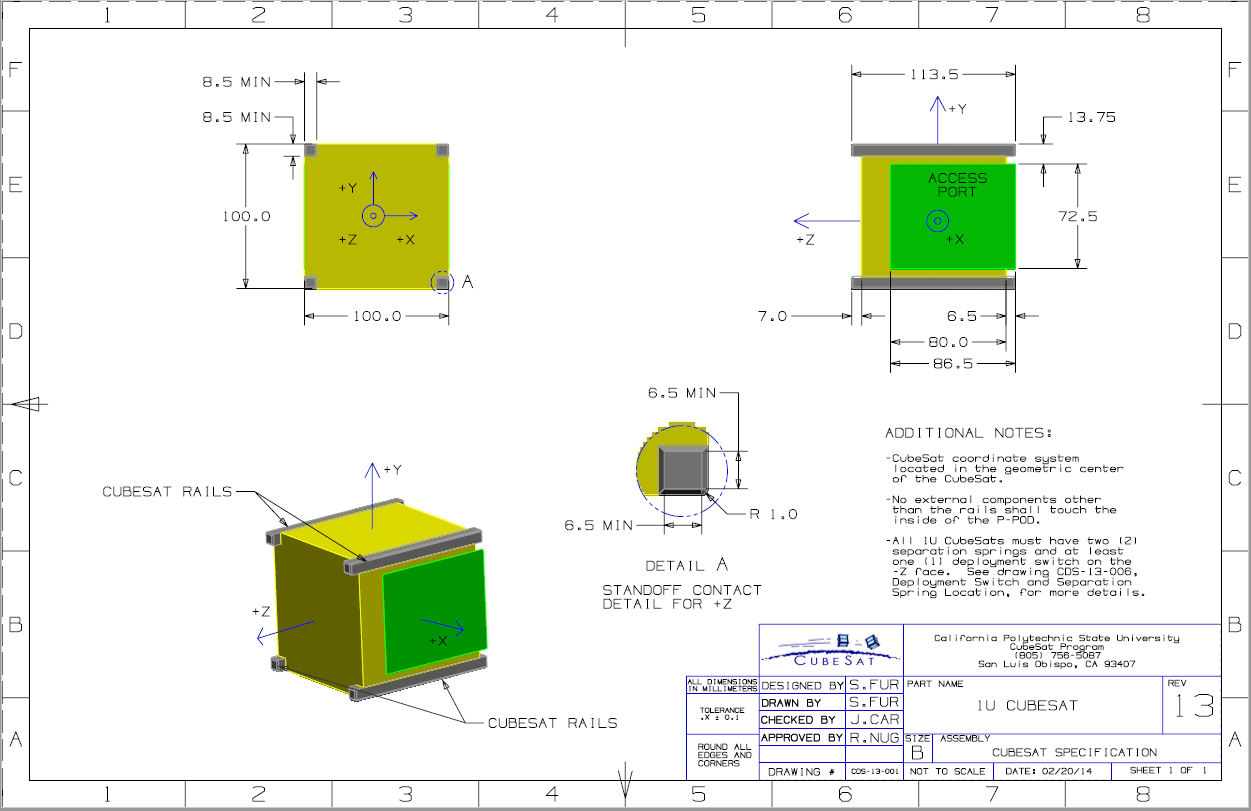
\includegraphics[keepaspectratio=true, scale=0.5]{imagens/Cubesat-diagram.png}}
% \captionof{figure}{Especificações de dimensionamento para um Cubesat 1U}
% \label{cubesat1U_dimensions}
% \end{minipage}

% A Tabela \ref{tabela1} a seguir apresenta os tipos de \textit{chunk} de um pacote do protocolo.

% \begin{table}[ht!]
%   \begin{center}
%   \setlength{\belowcaptionskip}{10pt} % espao entre caption e tabela
%   \footnotesize {
%       \begin{tabular}{|p{4cm}|p{9cm}|}
% 	  \hline
% 	  \textbf{Nome} & \textbf{Função} \\
% 	  \hline
% 	  Iniciar & Usado para iniciar uma associação \\
% 	  \hline
% 	  Confirmacao & Segunda mensagem de uma configuração de uma associação\\
% 	  \hline
% 	  Mensagem & Terceira mensagem de uma configuração de uma associação\\
% 	  \hline
% 	  Cookie & Quarta mensagem de uma configuração de uma associação\\
% 	  \hline
% 	  Dados & Dados da aplicação\\
% 	  \hline
%       \end{tabular}
%   }
%   \caption{Tipos de \textit{chunk} de um pacote SCTP}
%   \label{tabela1}
%   \end{center}
% \end{table}
